What is the equation of this circle if the center is at $(0,0)$ and point \textit{P} is at $(3,0)$?

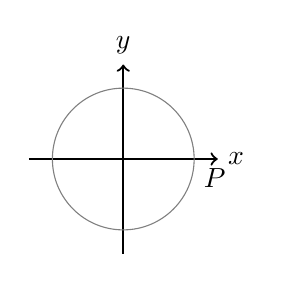
\begin{tikzpicture}[scale=0.6] 
\draw[->, thick](-2,0)--(2,0)node[anchor=west]{$x$}; 
\draw[->, thick](0,-2)--(0,2)node[anchor=south]{$y$}; 
\draw[gray](0,0)circle(1.5);  
\draw(1.5,0)node[anchor=north west]{$P$}; 
\end{tikzpicture} 

\ifsat
	\begin{enumerate}[label=\Alph*)]
		\item   $\textit{y}^2+\textit{x}^2=3$
		\item  $\textit{y}^2+\textit{x}^2=9$ % 
		\item  $\textit{y}^2+(\textit{x}-3)^2=3$ 
		\item  $\textit{y}^2+(\textit{x}-3)^2=9$ 
	\end{enumerate}
\else
\fi

\ifacteven
	\begin{enumerate}[label=\textbf{\Alph*.},itemsep=\fill,align=left]
		\setcounter{enumii}{5}
		\item   $\textit{y}^2+\textit{x}^2=3$
		\item  $\textit{y}^2+\textit{x}^2=9$ % 
		\item  $\textit{y}^2+(\textit{x}-3)^2=3$ 
		\addtocounter{enumii}{1}
		\item  $\textit{y}^2+(\textit{x}-3)^2=9$ 
		\item  $3\textit{y}^2+3\textit{x}^2=3$ 
	\end{enumerate}
\else
\fi

\ifactodd
	\begin{enumerate}[label=\textbf{\Alph*.},itemsep=\fill,align=left]
		\item   $\textit{y}^2+\textit{x}^2=3$
		\item  $\textit{y}^2+\textit{x}^2=9$ % 
		\item  $\textit{y}^2+(\textit{x}-3)^2=3$ 
		\item  $\textit{y}^2+(\textit{x}-3)^2=9$ 
		\item  $3\textit{y}^2+3\textit{x}^2=3$ 
	\end{enumerate}
\else
\fi

\ifgridin
  $\textit{y}^2+\textit{x}^2=9$ % 
		
\else
\fi

